\documentclass{beamer}




\usepackage[T1,T2A]{fontenc}
\usepackage[utf8]{inputenc}

\usepackage{graphicx}
\usepackage{blindtext}
\usepackage{ mathrsfs }
\usepackage[russian,english]{babel}

\author{Деркач Максим Юрьевич}
\title{Криптографические протоколы}
\subtitle{Лекция 3 \\ Управление ключами \\ Жизненый цикл ключей }
\setbeamercolor{frametitle}{bg=cyan!10}

%\usetheme{lucid}
\begin{document}
	\frame {
		\titlepage
	}
	\frame {
		\frametitle{Ссылки}
		
		\url{https://habr.com/ru/post/332730/}
		\url{https://habr.com/ru/post/475218/}
		
	}
	
	\frame {
		\frametitle{Управление ключами}
		\framesubtitle{Цель управления ключами}
	
		\textbf{Цель управления ключами} - нейтрализация следующих угроз:
	
		\begin{enumerate}
			\item компрометация конфиденциальности секретных ключей (СК).
			\item компрометация аутентичности секретных ключей (СК) и открытых ключей (ОК).
			\item несанкционированное использование секретных ключей (СК) и открытых ключей (ОК).
		\end{enumerate}
	
		\bigskip
	}
	
	\frame{
		\frametitle{Управление ключами}
		\framesubtitle{Политика безопасности}
	
		\textbf{Политика безопасности} определяет:
	
		\begin{enumerate}
			\item угрозы, которым должна противостоять система;
			\item правила и процедуры, которым необходимо руководствоваться в процессе управления ключами.
			\item ответственность и подотчетность всех субъектов, участвующих в управлении ключами.
			\item все виды записей, которые должны сохраняться.
		
		\end{enumerate}
	}


	\frame{
		\frametitle{Классификация ключей}
		\framesubtitle{Классификация ключей по значимости}
	
		\begin{enumerate}
			\item \textbf{Главный ключ} - не защищается криптографическими средствами,
			а для защиты применяются физические или организационные средства/методы;
			\item \textbf{Ключи шифрования ключей};
			\item \textbf{Ключи шифрования данных}.
		\end{enumerate}
	
	}
	
	\frame{
		\frametitle{Классификация ключей}
		\framesubtitle{Классификация ключей по сроку действия}
	
		Сокращение сроков действия ключей необходимо для достижения следующих целей:

		
		\begin{enumerate}
			\item ограничения объёма информации, зашифрованной на данном ключе, которая может быть использована для криптоанализа;

			\item ограничения размера ущерба при компрометации ключей;

			\item ограничения объёма машинного времени, которое может быть использовано для криптоанализа.
		\end{enumerate}
	
	\bigskip
		Классификация:
		\begin{enumerate}
			\item \textbf{Ключи с длительным сроком действия}: главный ключ и ключи для шифрования ключей;
			\item \textbf{Ключи с коротким сроком действия}: ключи для шифрования данных.
		\end{enumerate}
	}



\frame{
	\frametitle{Жизненный цикл ключей}
	
	\begin{enumerate}
		\item Регистрация пользователей системы: обмен первоначальной ключевой информацией (общие пароли, PIN-коды,...) путём физического обмена.
		\item Генерация ключей:
		\begin{itemize}
			\item Генерация ключей пользователями.
			\item Генерация ключей центром.
		\end{itemize}
		\item Установка ключей: устанавление ключей в оборудование тем или иным способом. 
		\item Регистрация ключей: Ключевая информация связывается регистрационным центром с именем пользователя и сообщается другим пользователям ключевой сети.
		\item Использование ключей.
		\item Хранение ключа защиты.
		\item Замена/обновление ключа: замена ключей до истечении срока использования.
		\end{enumerate}
		}

\frame{
	\frametitle{Жизненный цикл ключей}
	
	\begin{enumerate}
		\setcounter{enumi}{7}
		\item Архивирование ключа: ключ в дальнейшем не используется для шифрования данных или подписи,
		однако может быть использован для расшифрования старой информации.
		\item Восстановление ключа: если ключ был удален, но не скомпрометирован.
		\item Уничтожение ключа, в том числе информации по которой можно восстановить его: после окончания сроков действия ключей они выводятся из обращения, и все имеющиеся их копии уничтожаются.
		\item Отмена ключа, если ключ скомпрометирован: прекращение использования или отзыв сертификата.
	\end{enumerate}
}


\frame{
	\frametitle{Особенности управления ключами}
	\framesubtitle{Особенности управления ключами в симметричных к/c}
	
	\begin{itemize}
		\item Большое количество ключей: хранить неудобно и небезопасно.
		\item Для сокращения объема информации у обычного пользователя можно применить дополнительное распределение ключей.
		\item Представление сертификата секретных ключей: $cert_A = E_{K_S}(K_{AS}, ID_A, t)$, где t - срок действия сертификата.
	\end{itemize}

		\begin{enumerate}
			\item $A -> S: cert_A || E_{K_{AS}}(ID_B || M)||cert_B$
			\item $S -> A: E_{K_{BS}}(M||ID_A)$
			\item $A -> B: E_{K_{BS}}(M||ID_A)$
		\end{enumerate}	
	}

\frame{
	\frametitle{Особенности управления ключами}
	\framesubtitle{Особенности управления ключами в асимметричных к/c}
	
	\begin{itemize}
		\item Получение участниками сертификата:
		\begin{itemize}
			\item Пользователь сам генерирует пару ключей и запорашивает сертификат. Пользователь сам несет ответственность за генерацию.
			\item ТДС генерирует и создает сертификаты.
		\end{itemize}
		
		\item Отзыв сертификата.
		\item Большое число сертификатов у конечного пользователя.
	\end{itemize}
	
}

\frame{
	\frametitle{Особенности управления ключами}
	\framesubtitle{Процесс получения сертификата}

	\begin{figure}
		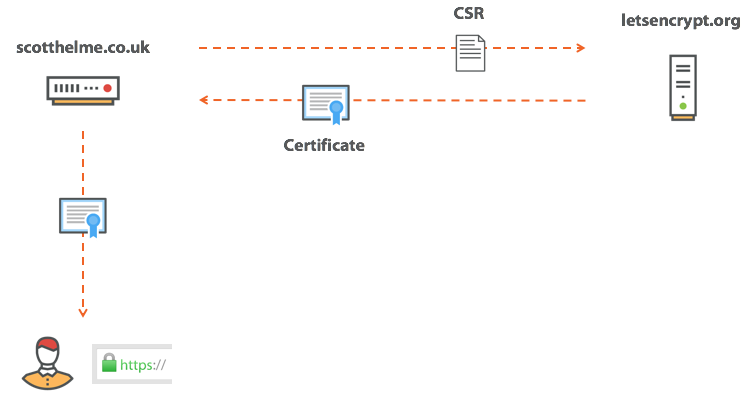
\includegraphics[width=0.8\linewidth]{csr.png}
	\end{figure}
}

\frame{
	\frametitle{Особенности управления ключами}
	\framesubtitle{Отзыв сертифката}
	
	\begin{figure}
		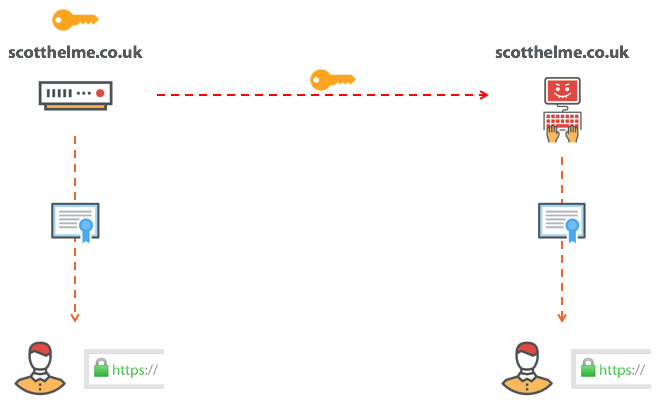
\includegraphics[width=0.8\linewidth]{hack.png}
	\end{figure}
}


\frame{
	\frametitle{Особенности управления ключами}
	\framesubtitle{Отзыв сертифката}
	
	\begin{figure}
		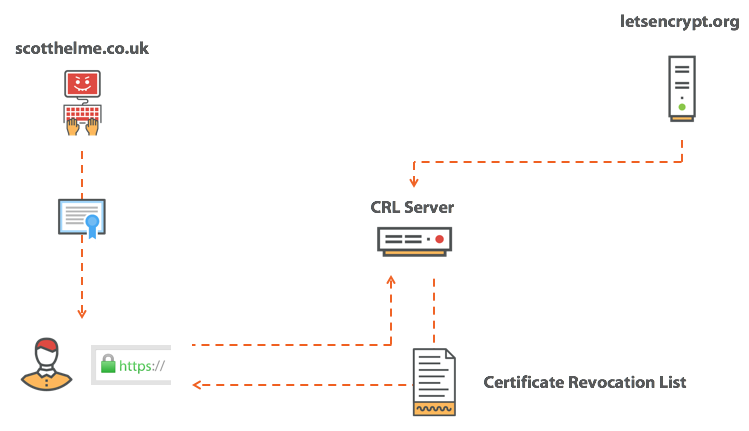
\includegraphics[width=0.8\linewidth]{crl.png}
	\end{figure}
}

\frame{
	\frametitle{Особенности управления ключами}
	\framesubtitle{Отзыв сертифката}
	
	\begin{figure}
		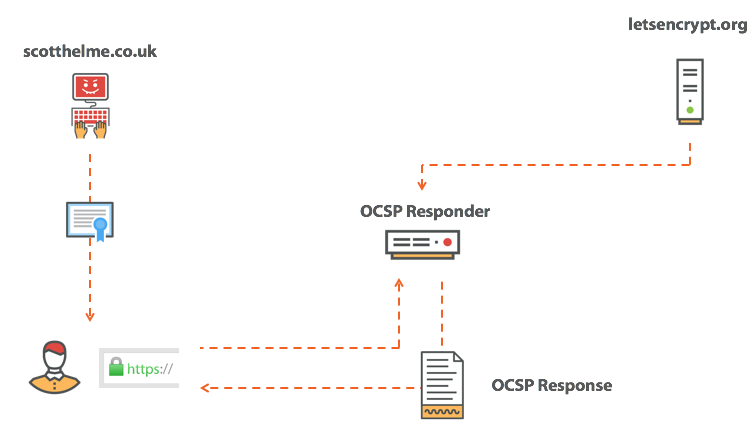
\includegraphics[width=0.8\linewidth]{ocsp.png}
	\end{figure}
}



\end{document}